\subsection*{Teil B: Punktsymmetrie (20 Minuten)}

\begin{merkbox}[Punktsymmetrie]
    Eine Figur ist \textbf{punktsymmetrisch}, wenn sie durch Drehung um 180° um einen Punkt (Symmetriezentrum) auf sich selbst abgebildet wird.
\end{merkbox}

\begin{enumerate}[label=\arabic*., resume]

    \item \textbf{Ergänze die Figur punktsymmetrisch zum Zentrum Z:}

    \vspace{0.5cm}

    \begin{center}
        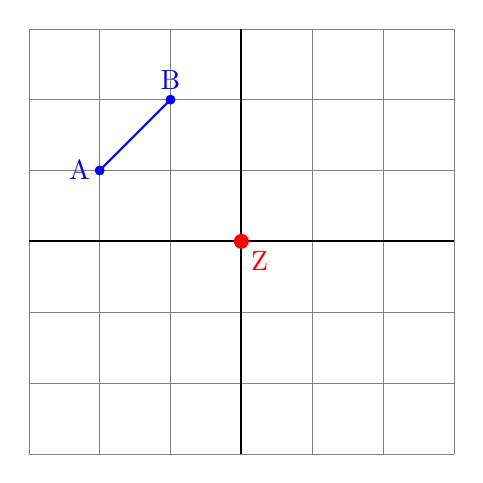
\begin{tikzpicture}[scale=0.9]
            % Koordinatensystem
            \draw[help lines] (-3,-3) grid (3,3);
            \draw[thick] (-3,0) -- (3,0);
            \draw[thick] (0,-3) -- (0,3);

            % Symmetriezentrum
            \fill[red] (0,0) circle (3pt) node[below right] {Z};

            % Gegebene Punkte
            \fill[blue] (-2,1) circle (2pt) node[left] {A};
            \fill[blue] (-1,2) circle (2pt) node[above] {B};
            \draw[thick, blue] (-2,1) -- (-1,2);
        \end{tikzpicture}
    \end{center}

    \vspace{1cm}

    \item \textbf{Welche Figuren sind punktsymmetrisch? Kreuze an:}

    \vspace{0.5cm}

    \begin{tabular}{|l|c|c|}
        \hline
        Figur & punktsymmetrisch & nicht punktsymmetrisch \\
        \hline
        Parallelogramm & $\square$ & $\square$ \\
        \hline
        Rechteck & $\square$ & $\square$ \\
        \hline
        Rhombus (Raute) & $\square$ & $\square$ \\
        \hline
        Gleichschenkliges Dreieck & $\square$ & $\square$ \\
        \hline
        Kreis & $\square$ & $\square$ \\
        \hline
    \end{tabular}

    \vspace{1cm}

    \item \textbf{Bestimme die Koordinaten der Bildpunkte bei Punktspiegelung am Ursprung:}

    Bei einer Punktspiegelung am Ursprung gilt: $P(x|y) \rightarrow P'(-x|-y)$

    \vspace{0.5cm}

    \begin{tabular}{|c|c|}
        \hline
        Urpunkt & Bildpunkt \\
        \hline
        $A(3|2)$ & $A'(\phantom{-0}|\phantom{-0})$ \\
        \hline
        $B(-1|4)$ & $B'(\phantom{-0}|\phantom{-0})$ \\
        \hline
        $C(0|-3)$ & $C'(\phantom{-0}|\phantom{-0})$ \\
        \hline
        $D(-2|-5)$ & $D'(\phantom{-0}|\phantom{-0})$ \\
        \hline
    \end{tabular}

\end{enumerate}